\section{Fourth strategy}

The purpose of this strategy is to find a better ordering of the graph $G$, on which we will use the activation strategy previously seen. We construct this order inductively (i.e. in the reverse order). The first selected node will be any vertex of $G$ with a degree of at most $5$.
Suppose we have already taken the vertices $v_{n}, v_{n-1}, ..., v_{i+1}$ except $v_{i}$ and we seek a candidate for $v_{i}$:

We split the vertices of $G$ into two parts: $C = (v_{n}, v_{n-1}, ..., v_{i+1})$ and $U = V \setminus C$.

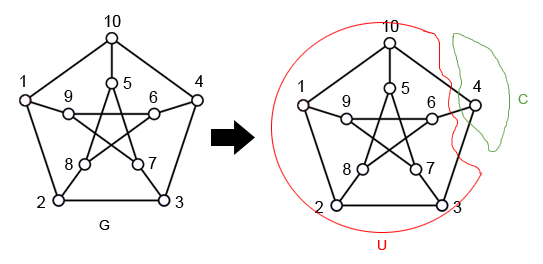
\includegraphics[width=10cm]{gameS4t1.jpg}

We construct a new graph $H$ as follows:
\begin{itemize}
\item We remove the edges between the vertices of C.
\item We remove each vertex $v$ of $C$ having at most three adjacent vertices in $U$.

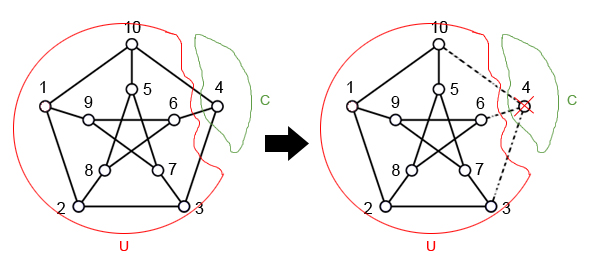
\includegraphics[width=10cm]{gameS4t2.jpg}

\item For each vertex $v$ removed, we add edges between its neighbors in $U$ in order to form a clique.

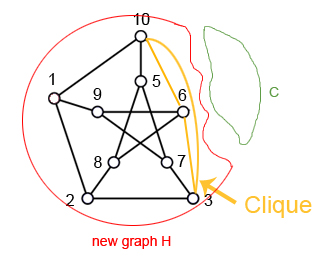
\includegraphics[width=6cm]{gameS4t3.jpg}

\end{itemize}

Now that we have our graph $H$, we assign to each edge $e$ 2 dollars (USD) spread over its vertices as follows:
\begin{itemize}
\item If $e$ connects two vertices of $U$, we give \$ 1 to each vertex of $e$.
\item If $e$ connects $x$ in $U$ and $y$ in $C$, then we give \$ 0.50 to $x$ and \$ 1.50 to $y$.

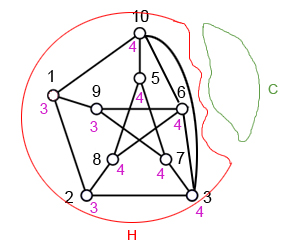
\includegraphics[width=5cm]{gameS4t4.jpg}

\end{itemize}

Once we have distributed the USD, we need to find a single vertex with a total value of less than \$ 6.
It will be our $v_{i}$.

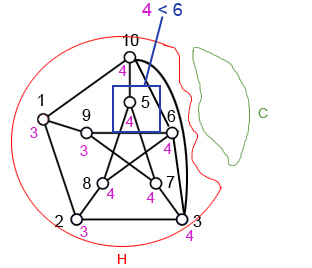
\includegraphics[width=6cm]{gameS4t5.jpg}

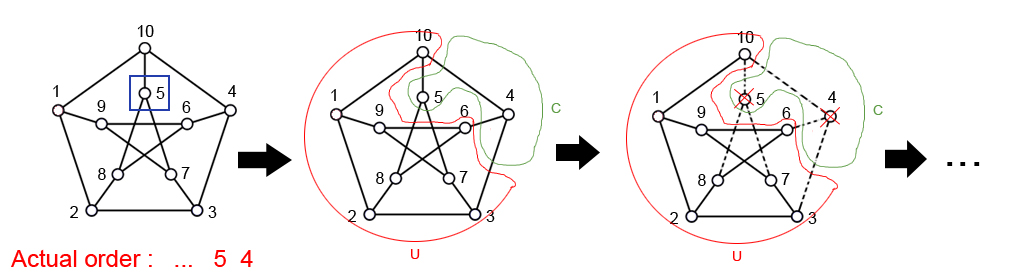
\includegraphics[width=15cm]{gameS4t6.jpg}

When we have our order, we use the color-blind activation strategy on it.

According to this strategy, every planar graph satisfies $\chi_{g}(G) \leq 18$.